\documentclass[10pt]{article}
% RATISS Labs — shared preamble (Tectonic / LaTeX)
\usepackage[a4paper,margin=2.3cm]{geometry}
\usepackage{xcolor}
\usepackage{graphicx}
\usepackage{booktabs}
\usepackage{amsmath}
\usepackage{microtype}
\usepackage[hidelinks]{hyperref}
\definecolor{ratiss}{RGB}{14,107,102}
\definecolor{ratisslight}{RGB}{238,252,249}
\definecolor{inkgray}{RGB}{74,111,107}
\hypersetup{colorlinks=true,linkcolor=ratiss,urlcolor=ratiss,citecolor=ratiss}
\setlength{\parindent}{0pt}
\setlength{\parskip}{5pt}
\renewcommand{\familydefault}{\sfdefault}
\newcommand{\ratisshead}[4]{%
  {\color{ratiss}\rule{\linewidth}{1.2pt}}\vspace{6pt}\\
  {\LARGE\bfseries #1}\\[4pt]
  {\large #2}\\[2pt]
  {\color{inkgray}\small #3}\\[2pt]
  {\color{inkgray}\small #4}\vspace{8pt}\\
  {\color{ratiss}\rule{\linewidth}{0.6pt}}\vspace{10pt}%
}
\newcommand{\kwsection}[1]{\section*{\color{ratiss}#1}\addcontentsline{toc}{section}{#1}}
\newcommand{\sourcefoot}{%
  \vspace{10pt}{\color{ratiss}\rule{\linewidth}{0.6pt}}\vspace{4pt}\\
  {\color{inkgray}\scriptsize RATISS Labs --- independent, single-author laboratory, Yaoundé (Cameroon).
  No number in this document is invented: every value carries a source in
  Section~``Data and code availability'' or in the references.
  Negative results are published with the same prominence as positive ones.}%
}

\begin{document}
\ratisshead
{Navier--Stokes Blow-up in 3D SPH with Tracers: Bit-for-Bit Reproducibility}
{Jonathan Evina --- RATISS Labs, Yaoundé, Cameroon}
{Research object \texttt{ratiss-navier-003} · revision 4 · 2026-10-02 · status: published}
{Repository: \url{https://github.com/jonathansearch/RATISS-NAVIER}}

\kwsection{Abstract}
A smoothed-particle hydrodynamics (SPH) study of vorticity growth up to blow-up,
in three dimensions, with lagrangian tracers. The blow-up value
$\Omega_{max} = 5654.1668$ reproduces bit-for-bit, with a pointwise gap of 0.0000
between independent runs. Four campaigns are published; revision 4 is sealed
(commit \texttt{8557fc6}).

\kwsection{Scientific question}
Is vorticity growth up to blow-up reproducible identically, run after run, on a
modest two-core machine?

\kwsection{Method}
3D SPH with lagrangian tracers; sampling at every time step; parameters frozen
\emph{before} execution in \texttt{PARAMETRES-FIGES.md}; full configuration embedded
in every campaign JSON. Criteria are sealed by the lab chief before any run.

\begin{figure}[h]\centering
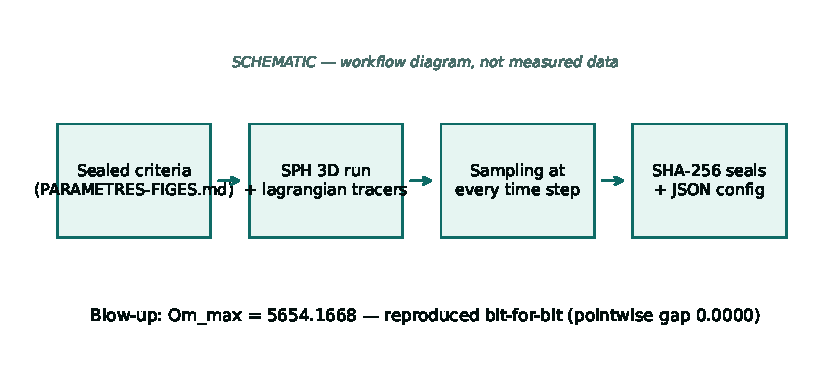
\includegraphics[width=0.95\linewidth]{fig/navier-workflow.pdf}
\caption{Verification workflow: sealed criteria, SPH run, per-step sampling, SHA-256
seals. Schematic diagram, not measured data.}\label{fig:workflow}
\end{figure}

\kwsection{Results}
\begin{itemize}
  \item Blow-up $\Omega_{max} = 5654.1668$, reproduced with pointwise gap 0.0000.
  \item Four published campaigns (last commit \texttt{5e736e0}); revision 4 sealed (\texttt{8557fc6}).
\end{itemize}

\kwsection{Negative results and open items}
\begin{itemize}
  \item V3 witnesses not rerun: the \texttt{dipoles-v3} criteria await the chief's signature.
  \item SPH resolution is limited by particle count; a numerical blow-up does not
        establish an analytic Navier--Stokes blow-up.
\end{itemize}

\kwsection{Controls}
Criteria sealed before runs; nothing pushed without an order; SHA-256 fingerprints of
outputs; cross-checked by the global test report (51/51 tests across six repositories).

\kwsection{Reproducibility}
Campaigns and frozen parameters live in \texttt{RATISS-NAVIER/campagnes/};
replay commands are documented per campaign.

\kwsection{Data and code availability}
\url{https://github.com/jonathansearch/RATISS-NAVIER};
test report: \texttt{RATISS-ARCHIVES/preuves/tests/RAPPORT-TESTS-RATISS.md}.
Zenodo DOI: to be assigned.

\sourcefoot
\end{document}
